\documentclass[14pt]{extarticle}
\usepackage[utf8]{inputenc}
\usepackage[T1]{fontenc}
\usepackage[spanish,es-lcroman]{babel}
\usepackage{amsmath}
\usepackage{amsthm}
\usepackage{physics}
\usepackage{tikz}
\usepackage{float}
\usepackage{cancel}
\usepackage[autostyle,spanish=mexican]{csquotes}
\usepackage[per-mode=symbol]{siunitx}
\usepackage{gensymb}
\usepackage{multicol}
\usepackage{enumitem}
\usepackage{stackengine}
\usepackage{stix}
\usepackage[left=2.00cm, right=2.00cm, top=2.00cm, 
     bottom=2.00cm]{geometry}

\usepackage{Estilos/ColoresLatex}
\usepackage{makecell}
\usepackage{wrapfig}

\newlength{\depthofsumsign}
\setlength{\depthofsumsign}{\depthof{$\sum$}}
\newcommand{\nsum}[1][1.4]{% only for \displaystyle
    \mathop{%
        \raisebox
            {-#1\depthofsumsign+1\depthofsumsign}
            {\scalebox
                {#1}
                {$\displaystyle\sum$}%
            }
    }
}

\newcommand{\textocolor}[2]{\textbf{\textcolor{#1}{#2}}}
%\renewcommand{\questionlabel}{\thequestion)}

\newcommand{\Cancel}[2][black]{{\color{#1}\cancel{\color{black}#2}}}

\newcommand\deci[1]{%
    \kern-.4ex\stackunder[0.4pt]{$#1$}{$\color{blue}\acwunderarcarrow$}
}

\newcommand\decposl[1]{%    <--- Decimal position to left
    \kern-.4ex\stackunder[0.4pt]{$#1$}{%
      \reflectbox{$\color{red}\kern-.6ex\acwunderarcarrow$}
      }
}

\renewcommand{\sin}{\operatorname{sen}}

\decimalpoint
\sisetup{bracket-numbers = false}

\title{\vspace*{-2cm} Guía de estudio Vectores  Física III}
\author{M. en C. Ramón Gustavo Contreras Mayén \\ {\fontsize{14}{14}\selectfont Universidad del Valle de México. Campus San Rafael}}
% \institute{Universidad del Valle de México. Campus San Rafael.}
\date{}

\begin{document}
\maketitle

\section{Descomposición de vectores}

En física hay cantidad que se expresan mediante vectores, recordemos que éstos se caracterizan por tres elementos: magnitud, dirección y sentido.

\subsection{Base geométrica.}

Consideremos un vector $\va{A}$ como se muestra a continuación:
\begin{figure}[H]
    \centering
    \begin{tikzpicture}[scale=1.2]
        \draw [-stealth, thick, color=blue] (0, 0) -- (2, 2) node [above, midway] {$\va{A}$};
        \draw (0.5, 0) arc(0:45:0.5);
        \node at (0.8, 0.2) {$\theta$};
        \draw (0, 0) -- (2.5, 0);
        \draw [-stealth, thick] (2, 0) -- (2, 2) node [right, midway] {$A_{y}$};
        \draw [-stealth, thick] (0, 0) -- (2, 0) node [below, midway] {$A_{x}$};
        \draw (1.8, 0) -- (1.8, 0.2) -- (2, 0.2);
    \end{tikzpicture}
\end{figure}

Las componentes del vector son:
\begin{align*}
A_{x} &= \cos \theta \, \abs{A} \\[0.5em] 
A_{y} &= \sin \theta \, \abs{A}
\end{align*}
Donde $\cos \theta$, es la función trigonométrica coseno del ángulo $\theta$ y la función $\sin \theta$, es la función también trigonométrica seno del ángulo $\theta$, por lo que se te recomienda apoyarte con el uso de una calculadora científica para obtener estos valores.

% \begin{figure}[H]
%     \centering
%     \begin{tikzpicture}[scale=1.3]
%         \draw [-stealth, thick, color=blue] (0, 0) -- (2, 2) node [above, midway] {$\va{A}$};
%         \draw (0.5, 0) arc(0:45:0.5);
%         \node at (0.8, 0.2) {$\theta$};
%         \draw (0, 0) -- (2.5, 0);
%         \draw [-stealth, thick] (2, 0) -- (2, 2) node [right, midway] {$A_{y}$};
%         \draw [-stealth, thick] (0, 0) -- (2, 0) node [below, midway] {$A_{x}$};
%         \draw (1.8, 0) -- (1.8, 0.2) -- (2, 0.2);
%     \end{tikzpicture}
% \end{figure}

La magnitud del vector $\va{A}$ es:
\begin{align*}
\abs{\va{A}} = \sqrt{(A_{x})^{2} + (A_{y})^{2}}
\end{align*}
que se obtiene del Teorema de Pitágoras, ya que se forma un triángulo rectángulo.
\begin{figure}[H]
    \centering
    \begin{tikzpicture}[scale=1.3]
        \draw [-stealth, thick, color=blue] (0, 0) -- (2, 2) node [above, midway] {$\va{A}$};
        \draw (0.5, 0) arc(0:45:0.5);
        \node at (0.8, 0.2) {$\theta$};
        \draw (0, 0) -- (2.5, 0);
        \draw [-stealth, thick] (2, 0) -- (2, 2) node [right, midway] {$A_{y}$};
        \draw [-stealth, thick] (0, 0) -- (2, 0) node [below, midway] {$A_{x}$};
        \draw (1.8, 0) -- (1.8, 0.2) -- (2, 0.2);
    \end{tikzpicture}
\end{figure}

La dirección del vector está dadar por el valor del ángulo $\theta$ es decir:
\begin{align*}
\theta = \tan^{-1} \left( \dfrac{A_y}{A_{x}} \right)
\end{align*}
La función $\tan^{-1}$ se lee: función tangente inversa o arcotangente.

\textbf{Ejercicio 1. } Calcula las componentes del siguiente vector:
\begin{figure}[H]
    \centering
    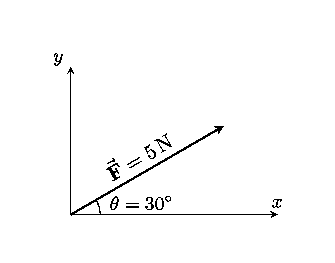
\includegraphics[scale=1.2]{Imagenes/Componentes_Vector_04.eps}
\end{figure}

Conocemos la magnitud del vector (\SI{5}{\newton}) y la dirección (el ángulo $\theta = \ang{30}$), por lo que hay que ocupar las expresiones:
\begin{align*}
F_{x} &= \cos \theta \, \abs{A} \\[0.5em] 
F_{y} &= \sin \theta \, \abs{A}    
\end{align*}

Para calcular la componente del vector en la dirección $x$, es decir $F_{x}$ sustituimos los valores 
\begin{align*}
F_{x} &= \cos \theta \, \abs{A} =  \\[0.5em] 
F_{x} &= \cos (\ang{30}) \cdot (\SI{5}{\newton}) =  \\[0.5em] 
F_{x} &= (0.866) (\SI{5}{\newton}) =  \\[0.5em] 
F_{x} &= \SI{4.33}{\newton}
\end{align*}

Para calcular la componente del vector en la dirección $y$, es decir, $F_{y}$, sustituimos los valores 
\begin{align*}
F_{y} &= \sin \theta \, \abs{A} =  \\[0.5em] 
F_{y} &= \sin (\ang{30}) \cdot (\SI{5}{\newton}) =  \\[0.5em] 
F_{y} &= (0.5) (\SI{5}{\newton}) =  \\[0.5em] 
F_{y} &= \SI{2.5}{\newton}
\end{align*}

\begin{figure}[H]
    \centering
    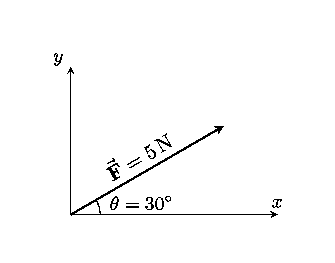
\includegraphics[scale=1.2]{Imagenes/Componentes_Vector_04.eps}
    \caption{Componentes del vector, recuerda indicar las unidades.}
\end{figure}
\begin{tikzpicture}[overlay]
    \node at (3, 5) {$F_{x} = \SI{4.33}{\newton}$};
    \node at (3, 4) {$F_{y} = \SI{2.5}{\newton}$};
\end{tikzpicture}

% \subsection{Vectores en otros cuadrantes}

% \begin{figure}
%     \centering
%     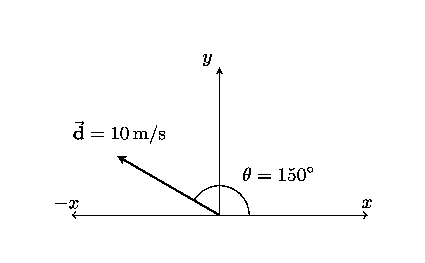
\includegraphics[scale=1.5]{Imagenes/Componentes_Vector_06.eps}
% \end{figure}


% Evaluando las funciones trigonométricas}
% Podríamos calcular las funciones trigonométricas seno y coseno del ángulo de 150 grados.

% \begin{eqnarray*}
% \begin{aligned}
% \cos \ang{150} &= -0.866 \\[0.5em] 
% \sin \ang{150} &= 0.5
% \end{aligned}
% \end{eqnarray*}


% Simplificando las cuentas}
% Recordando del curso de Matemáticas, aprovechamos mejor el ángulo suplementario, es decir,  el ángulo con el que se completan los 180 grados.


% Ángulo suplementario}
% \begin{figure}
%     \centering
%     \includegraphics[scale=1.5]{Imagenes/Componentes_Vector_07.eps}
% \end{figure}


% Detalle importante}
% Veamos que al calcular las funciones seno y coseno del ángulo suplementario, en el ejemplo $\varphi = \ang{30}$, obtenemos los valores:

% \begin{align*}
% \cos \ang{30} &= 0.866 \\[0.5em]
% \sin \ang{30} &= 0.5
% \end{align*}


% Detalle importante}
% Para la función coseno, el valor para el ángulo $\varphi = \ang{30}$, corresponde en magnitud que el valor del coseno de $\theta = \ang{150}$, pero NO le asocia es signo negativo.


% Detalle importante}
% Por lo que tendremos que anotar el signo negativo en la operación que corresponde para la componente en el eje $x$ de un vector.
% \\
% \bigskip

% La componente en el eje $x$, tiene su sentido en el eje $x$ negativo.



% Usando el ángulo suplementario}
% Una vez identificado el ángulo suplementario, procedemos a calcular las componentes del vector.

% \begin{eqnarray*}
% \begin{aligned}
% d_{x} &= - \cos \theta \, \abs{d} =  \\[0.5em] 
% &= - \cos (\ang{30}) \cdot (\SI[per-mode=symbol]{10}{\meter\per\second}) =  \\[0.5em] 
% &= - (0.866) (\SI[per-mode=symbol]{10}{\meter\per\second}) =  \\[0.5em] 
% &= - \SI[per-mode=symbol]{8.66}{\meter\per\second}
% \end{aligned}
% \end{eqnarray*}


% Usando el ángulo suplementario}
% Para la componente en el eje $y$ del vector $\va{d}$:

% \begin{eqnarray*}
% \begin{aligned}
% d_{y} &= \sin \theta \, \abs{d} =  \\[0.5em] 
% &= \sin (\ang{30}) \cdot (\SI[per-mode=symbol]{10}{\meter\per\second}) =  \\[0.5em] 
% &= (0.5) (\SI[per-mode=symbol]{10}{\meter\per\second}) =  \\[0.5em] 
% &= \SI[per-mode=symbol]{5}{\meter\per\second}
% \end{aligned}
% \end{eqnarray*}


% Revisión importante}
% Nota que la componente del vector en la dirección $x$, tiene un valor negativo.
% \\
% \bigskip
% Esto nos indica el sentido del vector, \textocolor{cobalt}{la magnitud siempre es un valor positivo}.


% ¿Qué pasa con los cuadrantes III y IV?}
% Al descomponer un vector, debes de verificar en qué cuadrante se encuentra,  ya que de esa manera, te dará una guía para determinar el signo de las componentes, como se vio en el caso de un vector en el cuadrante II.


% El cuadrante III}
% Considera que un vector en el cuadrante III, tendrá siempre la componente en el eje $x$ con un signo negativo,  y la componente en el eje $y$, también con signo negativo, como se muestra a continuación.


% El cuadrante III}
% \begin{figure}
%     \centering
%     \includegraphics[scale=1.25]{Imagenes/Componentes_Vector_08.eps}
% \end{figure}


% ¿Con qué ángulo se trabajaría en el cuadrante III?}
% Cuando tengamos un vector en el cuadrante III, podemos ocupar un ángulo complementario para simplificar las operaciones.


% El ángulo de trabajo}
% \begin{figure}
%     \centering
%     \includegraphics[scale=1.3]{Imagenes/Componentes_Vector_08a.eps}
% \end{figure}


% Las componentes del vector}
% Las componentes del vector $\va{C}$ en el cuadrante III, son entonces:
% \begin{align*}
% C_{x} & = - \cos \alpha \cdot \abs{\va{C}} \\[0.5em]
% C_{y} & = - \sin \alpha \cdot \abs{\va{C}}
% \end{align*}


% El cuadrante IV}
% Mientras que un vector en el cuadrante IV, tendrá siempre la componente en el eje $x$ con un signo positivo,  y la componente en el eje $y$, con signo negativo.


% El cuadrante IV}
% \begin{figure}
%     \centering
%     \includegraphics[scale=1.3]{Imagenes/Componentes_Vector_09.eps}
% \end{figure}


% Usando el ángulo complementario}
% Ahora consideramos el ángulo complementario en el cuadrante IV, como se muestra en la siguiente figura:


% Usando el ángulo complementario}
% \begin{figure}
%     \centering
%     \includegraphics[scale=1.3]{Imagenes/Componentes_Vector_09a.eps}
% \end{figure}


% Las componentes del vector}
% Las componentes del vector $\va{M}$ en el cuadrante IV, son entonces:
% \begin{align*}
% M_{x} & = \cos \psi \cdot \abs{\va{M}} \\[0.5em]
% M_{y} & = - \sin \psi \cdot \abs{\va{M}}
% \end{align*}

    
\subsection{El método analítico.}

Consideremos un conjunto de vectores, también conocido como \textocolor{islamicgreen}{sistema de vectores}:
\begin{align*}
\va{F}_{1}, \va{F}_{2}, \va{F}_{3}, \va{F}_{4}
\end{align*}
que están interactuando sobre un objeto.

Podemos considerar que sobre ese objeto actúa un solo vector,  que es la suma vectorial de esos vectores individuales:  \textocolor{red}{el vector resultante}.
\begin{align*}
\va{R} = \va{F}_{1} + \va{F}_{2} + \va{F}_{3} + \va{F}_{4} 
\end{align*}

El método analítico consiste en obtener el vector resultante, a partir de las componentes $F_{x}$, y $F_{y}$.

Sumando vectorialmente las componentes en cada eje, de cada vector, es decir:
\begin{align*}
R_{x} &= F_{1x} + F_{2x} + F_{3x} + F_{4x} =  \nsum_{i=1}^{4} F_{ix} \\[0.5em]  
R_{y} &= F_{1y} + F_{2y} + F_{3y} + F_{4y} =  \nsum_{i=1}^{4} F_{iy}
\end{align*}

Una vez obtenidas las componentes del vector resultante,  es posible calcular la magnitud del mismo, es decir $\abs{\va{R}}$:
\begin{align*}
\abs{\va{R}} = \sqrt{(R_{x})^{2} + (R_{y})^{2}}
\end{align*}

La última parte que nos falta, es determinar la dirección del vector, mediante el ángulo $\theta_{R}$ que forma con respecto al eje $x$ positivo, nos apoyamos con el uso de la función inversa de la tangente, que es la tangente inversa o arco tangente $\arctan$:
\begin{align*}
\tan \theta &= \dfrac{R_{y}}{R_{x}} \\[0.3em] 
\arctan(\tan \theta) &= \arctan(\dfrac{R_{y}}{R_{x}}) \\[0.5em] 
\theta &= \arctan(\dfrac{R_{y}}{R_{x}}) = \\[0.5em] 
\theta &= \tan^{-1} \left( \dfrac{R_{y}}{R_{x}} \right)
\end{align*}

\section*{Ejercicios a detalle.}

\subsection{Ejercicio 1.}

Calcula las componentes del siguiente vector.
\begin{figure}[H]
    \centering
    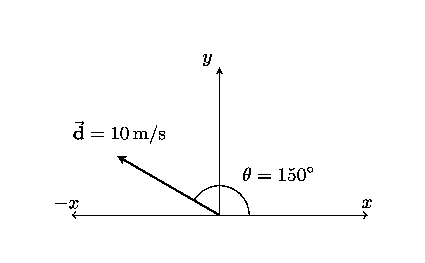
\includegraphics[scale=1.5]{Imagenes/Componentes_Vector_06.eps}
\end{figure}
Como se observa en la imagen, la cantidad que representa el vector $\va{d}$ es una velocidad, que siempre debemos de asociar en las componentes.

Calculamos las funciones trigonométricas seno y coseno del ángulo de \ang{150}.
\begin{align*}
\cos \ang{150} &= -0.866 \\[0.5em] 
\sin \ang{150} &= 0.5
\end{align*}

Por lo que la componente en $d_{x}$ en la dirección del eje de las abscisas o eje de las $x$, es:
\begin{align*}
d_{x} &= \cos \theta \, \abs{\va{d}} =  \\[0.5em]
d_{x} &= \cos (\ang{150}) \cdot (\SI[per-mode=symbol]{10}{\meter\per\second}) = \\[0.5em]
d_{x} &=  (-0.866) (\SI[per-mode=symbol]{10}{\meter\per\second}) = \\[0.5em]
d_{x} &= - \SI[per-mode=symbol]{8.66}{\meter\per\second}
\end{align*}

Para la componente $d_{y}$ en el eje de las ordenadas, o llamado también el eje $y$:
\begin{align*}
d_{y} &= \sin \theta \, \abs{\va{d}} = \\[0.5em] 
d_{y} &= \sin (\ang{150}) \cdot (\SI[per-mode=symbol]{10}{\meter\per\second}) = \\[0.5em] 
d_{y} &= (0.5) (\SI[per-mode=symbol]{10}{\meter\per\second}) = \\[0.5em] 
d_{y} &= \SI[per-mode=symbol]{5}{\meter\per\second}
\end{align*}

\subsection{Ejercicio 2.}

Realiza la descomposición del siguiente vector $\va{A}$:
\begin{figure}[H]
    \centering
    \begin{tikzpicture}[scale=2.5]
        \draw [-stealth] (-1, 0) -- (1, 0) node [above, pos=1] {$x$};
        \draw [-stealth] (0, -1) -- (0, 1) node [left, pos=1] {$y$};
        \node at (-1, -0.15) {$-x$};
        \node at (0.2, -1) {$-y$};
        \draw [-stealth, thick] (0, 0) -- (-0.342, -0.939);
        \node at (-0.75, -0.5) {$\va{A} = \SI{2}{\newton}$};
        \draw [-stealth] (0.2, 0) arc(0:250:0.2);
        \node at (-0.5, 0.2) {\small{$\theta = \ang{250}$}};
    \end{tikzpicture}
\end{figure}
Simplificamos la tarea mediante una tabla:
\begin{table}[H]
\centering
\begin{tabular}{c | l | l | c}
Componente & Expresión & Sustitución & Valor \\ \hline
$A_{x}$ & $\cos \ang{250} \cdot \va{A}$ & $(-0.3420) \cdot \SI{2}{\newton}$ & $\SI{-0.6840}{\newton}$ \\ \hline
$A_{y}$ & $\sin \ang{250} \cdot \va{A}$ & $(-0.9396) \cdot \SI{2}{\newton}$ & $\SI{-1.8793}{\newton}$ \\ \hline
\end{tabular}
\end{table}
Por lo que las componentes del vector $\va{A}$ son:
\begin{align*}
A_{x} &= \SI{-0.6840}{\newton} \\
A_{y} &= \SI{-1.8793}{\newton}
\end{align*}

\subsection{Ejercicio 2.}

Realiza la descomposición del siguiente vector $\va{B}$.
\begin{figure}[H]
    \centering
    \begin{tikzpicture}[scale=1.5]
        \draw [-stealth] (-0.5, 0) -- (2.5, 0) node [above, pos=1] {$x$};
        \draw [-stealth] (0, 0.5) -- (0, -3.5) node [left, pos=1] {$-y$};
        \draw [-stealth, thick] (0, 0) -- (2, -3.46);
        \node at (1.5, -1) {$\va{B} = \SI{4}{\newton}$};
        \draw [-stealth] (0.3, 0) arc(0:300:0.3);
        \node at (1.2, 0.2) {$\theta = \ang{300}$};
    \end{tikzpicture}
\end{figure}

Nuevamente simplificamos la tarea mediante una tabla:
\begin{table}[H]
\centering
\begin{tabular}{c | l | l | c}
Componente & Expresión & Sustitución & Valor \\ \hline
$B_{x}$ & $\cos \ang{300} \cdot \va{A}$ & $(0.5) \cdot \SI{4}{\newton}$ & $\SI{2}{\newton}$ \\ \hline
$B_{y}$ & $\sin \ang{300} \cdot \va{A}$ & $(-0.866) \cdot \SI{4}{\newton}$ & $\SI{-3.4641}{\newton}$ \\ \hline
\end{tabular}
\end{table}
Por lo que las componentes del vector $\va{A}$ son:
\begin{align*}
B_{x} &= \SI{2}{\newton} \\
B_{y} &= \SI{-3.4641}{\newton}
\end{align*}

\subsection{Ejercicio .}

Del siguiente sistema de vectores determina por el método analítico el valor de la magnitud $\abs{R}$ del vector resultante y el ángulo que forma con respecto al eje $x$ positivo, es decir, el ángulo $\theta_{R}$.

\begin{figure}[H]
\centering
\begin{tikzpicture}[scale=0.8]
    \draw (-4, 0) -- (9, 0) node [above, pos=1] {$x$};
    \draw (0, -4) -- (0, 6) node [left, pos=1] {$y$};
    \node at (-4, 0.3) {$-x$};
    \node at (0.4, -4) {$-y$};
    \draw [-stealth, line width=0.5mm, color=blue] (0, 0) -- (8, 0) node [below, midway] {$\va{F}_{1} = \SI{8}{\newton}$};
    \draw [-stealth, line width=0.5mm, color=burgundy] (0, 0) -- (4.59, 3.85) node [above, near end, rotate=40] {$\va{F}_{2} = \SI{6}{\newton}$};
    \draw [color=burgundy] (0.5, 0) arc(0:40:0.5);
    \node [color=burgundy] at (2, 0.4) {$\theta_{2} = \ang{40}$};
    \draw [-stealth, line width=0.5mm, color=cerise] (0, 0) -- (-2.59, -1.5) node [below, near end, rotate=30] {$\va{F}_{3} = \SI{3}{\newton}$};
    \draw [color=cerise] (-0.5, 0) arc(180:210:0.5);
    \node [color=cerise] at (-2,- 0.3) {$\theta_{3} = \ang{30}$};
    \draw [-stealth, line width=0.5mm, color=byzantine] (0, 0) -- (0, 5) node [left, near end] {$\va{F}_{4} = \SI{5}{\newton}$};
\end{tikzpicture}
\end{figure}

\textbf{Recomendación para la solución. } Es conveniente enlistar los vectores involucrados de tal manera que tengamos identificado cada vector, así como su magnitud y el ángulo.

Recordemos que todo vector debe de tener un ángulo asociado, veremos en particular que en el ejercicio hay dos vectores que coinciden con los ejes del sistema cartesiano, el vector $F_{3}$ forma un ángulo de \ang{30} con respecto al eje horizantal $-x$, en este caso podemos resolver las componentes $F_{3x}$ y $F_{3y}$ de dos maneras que veremos a continuación.

\textocolor{ao}{Lista de vectores.}
\begin{table}[H]
\centering
\begin{tabular}{c | c | c }
Vector & Magnitud (en $\unit{\newton}$) & Ángulo \\ \hline
$\va{F}_{1}$ & $8$ & $\theta_{1} = \ang{0}$ \\ \hline
$\va{F}_{2}$ & $6$ & $\theta_{2} = \ang{40}$ \\ \hline
$\va{F}_{3}$ & $3$ & $\theta_{3} = \ang{30}$ \\ \hline
$\va{F}_{4}$ & $5$ & $\theta_{4} = \ang{90}$ \\ \hline
\end{tabular}
\end{table}

Una vez que tenemos la lista de vectores, iniciamos el cálculo de las componentes $F_{x}$ y $F_{y}$ de cada uno de ellos. Se recomienda también hacer una tabla con las componentes.

\textocolor{byzantine}{Tabla con las componentes.}
\begin{table}[H]
\centering
\begin{tabular}{c | l | l | c}
Componente & Expresión & Sustitución & Valor \\ \hline
$F_{1x}$ & $\cos \theta_{1} \cdot F_{1}$ & $\cos \ang{0} \cdot \SI{8}{\newton}$ & $\SI{8}{\newton}$ \\ \hline
$F_{1y}$ & $\sin \theta_{1} \cdot F_{1}$ & $\sin \ang{0} \cdot \SI{8}{\newton}$ & $\SI{0}{\newton}$ \\ \hline
$F_{2x}$ & $\cos \theta_{2} \cdot F_{2}$ & $\cos \ang{40} \cdot \SI{6}{\newton}$ & $\SI{4.59}{\newton}$ \\ \hline
$F_{2y}$ & $\sin \theta_{2} \cdot F_{2}$ & $\sin \ang{40} \cdot \SI{6}{\newton}$ & $\SI{3.85}{\newton}$ \\ \hline
$F_{3x}$ & $-\cos \theta_{3} \cdot F_{3}$ & $-\cos \ang{30} \cdot \SI{3}{\newton}$ & $-\SI{2.59}{\newton}$ \\ \hline
$F_{3y}$ & $-\sin \theta_{3} \cdot F_{3}$ & $-\sin \ang{30} \cdot \SI{3}{\newton}$ & $-\SI{1.5}{\newton}$ \\ \hline
$F_{4x}$ & $\cos \theta_{4} \cdot F_{4}$ & $\cos \ang{90} \cdot \SI{5}{\newton}$ & $\SI{0}{\newton}$ \\ \hline
$F_{4y}$ & $\sin \theta_{4} \cdot F_{4}$ & $\sin \ang{90} \cdot \SI{5}{\newton}$ & $\SI{5}{\newton}$ \\ \hline
\end{tabular}
\end{table}

Notemos que el vector $F_{3}$ está en el cuadrante III, por lo que las componentes tanto en la dirección $x$, como en la dirección $y$, tienen un signo negativo. Si usamos la geometría plana, llegaremos a las componentes en $x$ y en $y$ de este vector.

\begin{figure}[H]
\centering
\begin{tikzpicture}[scale=0.8]
    \draw (-4, 0) -- (9, 0) node [above, pos=1] {$x$};
    \node at (-4, 0.3) {$-x$};
    \draw (0, -4) -- (0, 6) node [left, pos=1] {$y$};
    \node at (-0.6, -4) {$-y$};
    % \draw [-stealth, line width=0.5mm, color=blue] (0, 0) -- (8, 0) node [below, midway] {$\va{F}_{1} = \SI{8}{\newton}$};
    % \draw [-stealth, line width=0.5mm, color=burgundy] (0, 0) -- (4.59, 3.85) node [above, near end, rotate=40] {$\va{F}_{2} = \SI{6}{\newton}$};
    % \draw [color=burgundy] (0.5, 0) arc(0:40:0.5);
    % \node [color=burgundy] at (2, 0.4) {$\theta_{2} = \ang{40}$};
    \draw [-stealth, line width=0.5mm, color=cerise] (0, 0) -- (-2.59, -1.5) node [below, near end, rotate=30] {$\va{F}_{3} = \SI{3}{\newton}$};
    \draw [color=cerise] (-0.5, 0) arc(180:210:0.5);
    \node [color=cerise] at (-2,- 0.3) {\small{$\theta_{3} = \ang{30}$}};

    \draw [color=ao] (0.5, 0) arc(0:210:0.5);
    \node [color=ao] at (1.3, 0.7) {\small{$\theta_{3} = \ang{210}$}};
    % \draw [-stealth, line width=0.5mm, color=byzantine] (0, 0) -- (0, 5) node [left, near end] {$\va{F}_{4} = \SI{5}{\newton}$};
\end{tikzpicture}
\end{figure}
Hagamos la operación con los dos ángulos:
\begin{table}[H]
\centering
\begin{tabular}{c | l | l | c}
Componente & Ángulo & Sustitución & Valor \\ \hline
$F_{3x}$ & $\theta_{3} = \ang{30}$ & $-\cos \ang{30} \cdot \SI{3}{\newton}$ & $-\SI{2.59}{\newton}$ \\ \hline
$F_{1y}$ & $\theta_{3} = \ang{30}$ & $-\sin \ang{30} \cdot \SI{3}{\newton}$ & $-\SI{1.5}{\newton}$ \\ \hline
$F_{3x}$ & $\theta_{3} = \ang{210}$ & $\cos \ang{210} \cdot \SI{3}{\newton}$ & $-\SI{2.59}{\newton}$ \\ \hline
$F_{1y}$ & $\theta_{3} = \ang{210}$ & $\sin \ang{210} \cdot \SI{3}{\newton}$ & $-\SI{1.5}{\newton}$ \\ \hline
\end{tabular}
\end{table}
Encontramos que el valor de las componentes es el mismo, sin importar el ángulo que hayamos elegido, pero toma en cuenta de que si hacemos uso del ángulo de la figura, es decir, \ang{30}, debemos de anotar manualmente el signo negativo para que la componente mantenga ese signo.

Ahora ya podemos calcular las componentes del vector resultante,  recordemos que la componente en la dirección $x$ es:
\begin{align*}
R_{x} &= \nsum_{i=1}^{4} F_{ix} =  F_{1x} + F_{2x} + F_{3x} + F_{4x} = \\[0.5em] 
&= \SI{8}{\newton} {+} \SI{4.59}{\newton} {+} (-\SI{2.59}{\newton}) {+} \SI{0}{\newton} = \\[0.5em] 
&= \SI{10}{\newton}
\end{align*}

Para la componente en la dirección $y$ del vector resultante $R_{y}$:
\begin{align*}
R_{y} &= \nsum_{i=1}^{4} F_{iy} =  F_{1y} + F_{2y} + F_{3y} + F_{4y} = \\[0.5em] 
R_{y} &= \SI{0}{\newton} {+} \SI{3.85}{\newton} {+} (-\SI{1.5}{\newton}) {+} \SI{5}{\newton} = \\[0.5em] 
R_{y} &= \SI{7.35}{\newton}
\end{align*}

Una vez obtenidas las componentes en $x$ e $y$, calculamos la magnitud del vector resultante $\abs{\va{R}}$:
\begin{align*}
\abs{\va{R}} &= \sqrt{(R_{x})^{2} + (R_{y})^{2}} = \\[0.5em] 
\abs{\va{R}} &= \sqrt{(\SI{10}{\newton})^{2} + (\SI{7.35}{\newton})^{2}} = \\[0.5em] 
\abs{\va{R}} &= \sqrt{\SI{100}{\square\newton} + \SI{54.02}{\square\newton}} =  \sqrt{\SI{154.02}{\square\newton}} = \\[0.5em] 
\abs{\va{R}} &= \SI{12.41}{\newton}
\end{align*}

Tenemos que $R_{x} > 0$ y $R_{y} > 0$,  por lo que el vector resultante está en el cuadrante I,  con esos valores podemos calcular el valor del ángulo del vector resultante con respecto al eje $x$ positivo.  El ángulo $\theta_{R}$ resulta ser:
\begin{align*}
\tan \theta_{R} &= \dfrac{R_{y}}{R_{x}} = 
    \dfrac{\SI{7.35}{\newton}}{\SI{10}{\newton}} =   0.735 \\[0.5em] 
\arctan(\tan \theta_{R}) &= \arctan(0.735) \\[0.5em] 
\theta_{R} &= \ang{36.31}
\end{align*}

Conocida la información del vector $\va{R}$, lo representamos en el sistema cartesiano.
\begin{figure}[H]
\centering
\begin{tikzpicture}[scale=0.5]
    \draw (-4, 0) -- (9, 0) node [above, pos=1] {$x$};
    \draw (0, -4) -- (0, 6) node [left, pos=1] {$y$};
    \draw [-stealth, thick, color=blue] (0, 0) -- (8, 0) node [below, midway] {\small{$\va{F}_{1}$}};

    \draw [-stealth, thick, color=burgundy] (0, 0) -- (4.59, 3.85) node [above, near end, rotate=40] {\small{$\va{F}_{2}$}};
    \draw [color=burgundy] (0.5, 0) arc(0:40:0.5);
    \node [color=burgundy] at (1.6, 0.4) {\small{$\theta_{2}$}};

    \draw [-stealth, thick, color=cerise] (0, 0) -- (-2.59, -1.5) node [below, near end, rotate=30] {\small{$\va{F}_{3}$}};
    \draw [color=cerise] (-0.5, 0) arc(180:210:0.5);
    \node [color=cerise] at (-1.8,- 0.4) {\small{$\theta_{3}$}};

    \draw [-stealth, thick, color=byzantine] (0, 0) -- (0, 5) node [left, near end] {\small{$\va{F}_{4}$}};
    
    \draw [-stealth, line width=0.5mm, color=cadmiumred] (0, 0) -- (9.69, 7.35) node [above, near end, rotate=37] {\small{$\va{R} = \SI{12.41}{\newton}$}};
    \draw [thick, color=cadmiumred] (3, 0) arc(0:37:3);
    \node [color=cadmiumred] at (5.2, 0.8) {\small{$\theta_{R} = \ang{36.31}$}};
\end{tikzpicture}
\caption{El vector resultante del sistema de vectores.}
\end{figure}

\end{document}